\documentclass[a4paper]{article}

%use the english line for english reports
%usepackage[english]{babel}
\usepackage[portuguese]{babel}
\usepackage[utf8]{inputenc}
\usepackage{indentfirst}
\usepackage{graphicx}
\usepackage{verbatim}
\usepackage{listings}


\begin{document}

\setlength{\textwidth}{16cm}
\setlength{\textheight}{22cm}

\title{\Huge\textbf{Syrtis}\linebreak\linebreak\linebreak
\Large\textbf{Relatório Intercalar}\linebreak\linebreak
\linebreak\linebreak

\includegraphics[scale=0.1]{feup-logo.png}\linebreak\linebreak
\linebreak\linebreak
\Large{Mestrado Integrado em Engenharia Informática e Computação} \linebreak\linebreak
\Large{Programação em Lógica}\linebreak
}

\author{\textbf{Grupo 79:}\\
Flávio Couto - 201303726 \\
Pedro Afonso Castro - 201304205 \\
\linebreak\linebreak \\
 \\ Faculdade de Engenharia da Universidade do Porto \\ Rua Roberto Frias, s\/n, 4200-465 Porto, Portugal \linebreak\linebreak\linebreak
\linebreak\linebreak\vspace{1cm}}

\maketitle
\thispagestyle{empty}

%************************************************************************************************
%************************************************************************************************

\newpage

%Todas as figuras devem ser referidas no texto. %\ref{fig:codigoFigura}
%
%%Exemplo de código para inserção de figuras
%%\begin{figure}[h!]
%%\begin{center}
%%escolher entre uma das seguintes três linhas:
%%\includegraphics[height=20cm,width=15cm]{path relativo da imagem}
%%\includegraphics[scale=0.5]{path relativo da imagem}
%%\includegraphics{path relativo da imagem}
%%\caption{legenda da figura}
%%\label{fig:codigoFigura}
%%\end{center}
%%\end{figure}
%
%
%\textit{Para escrever em itálico}
%\textbf{Para escrever em negrito}
%Para escrever em letra normal
%``Para escrever texto entre aspas''
%
%Para fazer parágrafo, deixar uma linha em branco.
%
%Como fazer bullet points:
%\begin{itemize}
	%\item Item1
	%\item Item2
%\end{itemize}
%
%Como enumerar itens:
%\begin{enumerate}
	%\item Item 1
	%\item Item 2
%\end{enumerate}
%
%\begin{quote}``Isto é uma citação''\end{quote}


%%%%%%%%%%%%%%%%%%%%%%%%%%
\section{Introdução}

O principal objetivo deste projeto é adquirir competências ao nível da Programação em Lógica através do estudo de um jogo de tabuleiro previamente escolhido. Foram-nos dadas várias hipóteses de jogos, tendo nós escolhido o Syrtis, por causa da sua elevada componente estratégica e tática, bem como alguma complexidade, sempre necessária para trazer um maior sentimento de desafio quando nos é colocado um projeto em mãos.

\section{O Jogo Syrtis}

Segue-se uma explicação das regras do Syrtis, bem como alguns exemplos para melhor demonstrar alguns aspetos que possam ser de maior dificuldade de compreensão.

\subsection{História}

	O Syris é um jogo de estratégia em que os dois jogadores se encontram numa ilha instável e desconhecida. A paisagem da ilha está sempre em mudança, e o avanço do mar faz com que a ilha esteja a tornar-se cada vez mais pequena... Para complicar ainda mais, este avanço está a fazer com que se formem areias movediças, limitando ainda mais o espaço habitável na ilha... Apenas um dos jogadores poderá sobreviver, quem será capaz de ser o mais forte?
	
\subsection{Objetivo}
	
	A cada jogador é atribuída uma forma e uma cor (quadrado e preto ou círculo e branco). O objetivo do jogo é conquistar todas as peças que contenham a sua cor ou a sua forma.
	
\subsection{Equipamento}

	O jogo é composto por peças quadradas com uma determinada forma e cor. Há 4 combinações possíveis: círculos e quadrados brancos e pretos. Há também quatro torres, duas brancas e circulares e duas pretas e quadradas.
	
\subsection{Preparação}

	As peças quadradas são inicialmente aleatoriamente dispostas num de dois formatos de ilha. Para um jogo mais longo e estratégico, utiliza-se o formato Syrtis Major. Para um jogo mais curto e tático, utiliza-se o formato Syrtis Minor. As figuras \ref{fig:syrtismajor} e \ref{fig:syrtisminor} mostram a estrutura destes dois formatos.
	
\begin{figure}[h]

\begin{minipage}{0.5\linewidth}
\centering
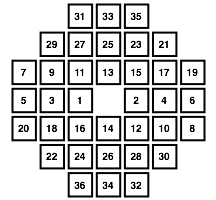
\includegraphics[scale=0.9]{syrtismajor.png}
\caption{Syrtis Major}
\label{fig:syrtismajor}
\end{minipage}
\quad
\begin{minipage}{0.5\linewidth}
\centering
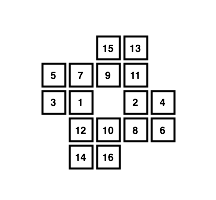
\includegraphics[scale=0.9]{syrtisminor.png}
\caption{Syrtis Minor}
\label{fig:syrtisminor}
\end{minipage}

\end{figure}

Depois, um dos jogadores coloca as 4 torres por cima de uma das peças à sua escolha, desde que sejam da cor ou da forma dessa peça. O outro jogador decide se quer jogar com as torres brancas circulares ou pretas quadradas e o jogo começa por quem tiver ficado com as peças brancas e circulares.

\subsection{Ilhas}

Uma ilha é uma peça ou um grupo de peças que partilham a mesma forma ou cor. Para serem consideradas uma ilha, devem estar adjacentes horizontal ou verticalmente. Há quatro tipos de ilhas: ilhas pretas, brancas, quadradas e circulares. Uma peça pode obviamente pertencer a uma ilha de uma cor e a uma ilha de uma forma ao mesmo tempo. As figuras \ref{fig:circleisland} e \ref{fig:blackisland} mostram exemplos de ilhas.

\begin{figure}[h]

\begin{minipage}{0.5\linewidth}
\centering
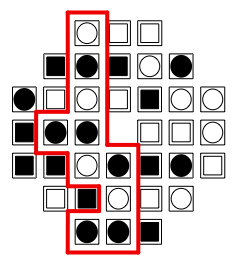
\includegraphics[scale=0.75]{island1.png}
\caption{Ilha de círculos}
\label{fig:circleisland}
\end{minipage}
\quad
\begin{minipage}{0.5\linewidth}
\centering
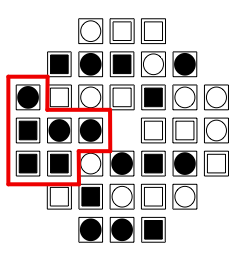
\includegraphics[scale=0.75]{island2.png}
\caption{Ilha de pretos}
\label{fig:blackisland}
\end{minipage}

\end{figure}


\subsection{Acções}
\label{sec:actions}

Em cada turno cada jogador pode fazer uma de entre 4 acções possíveis: mover uma torre, afundar uma peça, deslocar uma peça, ou passar a sua vez.

\subsubsection{Mover uma torre}

Cada jogador pode mover uma das suas torres, desde que se mantenha em pelo menos uma das suas duas ilhas atuais (ou seja, ou na ilha respeitante à forma ou na ilha respeitante à cor). As outras torres não bloqueiam este movimento, ou seja, podemos passar por cima de outras torres.  A figura \ref{fig:towermovement} mostra um exemplo do movimento de uma torre.

\begin{figure}[h]
\centering
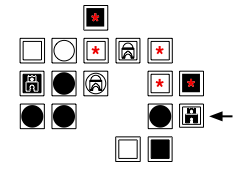
\includegraphics[scale=0.9]{towermovement.png}
\caption{Movimento de uma torre}
\label{fig:towermovement}
\end{figure}

A torre indicada (preta e quadrada) pode mover-se para qualquer uma das peças marcadas com uma seta, pois estas encontram-se na sua ilha quadrangular. Note-se também que ela não pode ir para a peça à sua esquerda, visto que, apesar de ser preta, esta não se encontra na sua ilha (visto que a peça em que a torre se encontra é branca e quadrada, e a peça em questão é preta e circular).

\subsubsection{Afundar uma peça}

Cada jogador pode remover uma peça do tabuleiro se:

\begin{itemize}
\item Esta for adjacente a uma peça ocupada por uma torre desse jogador;
\item Esta estiver desocupada;
\item Esta tiver pelo menos um espaço adjacente livre.
\end{itemize}

A figura \ref{fig:sinktile} mostra um exemplo de quais peças podem ser afundadas.

\begin{figure}[h]
\centering
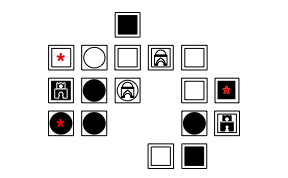
\includegraphics[scale=0.9]{sinktile.png}
\caption{Peças afundáveis}
\label{fig:sinktile}
\end{figure}


O jogador preto pode afundar quaisquer peças que estejam marcadas com uma estrela. Nenhuma peça branca está numa posição que lhe permita afundar alguma peça.

\subsubsection{Deslocar uma peça}

Um jogador poderá deslocar uma peça ocupada por uma das suas torres através de quaisquer espaços vazios que estejam conectados. A peça pode ser movida em qualquer direcção, quantas vezes quisermos, desde que a largura ou altura do tabuleiro não seja aumentada (nem mesmo a meio do movimento) e as peças do tabuleiro continuem conectadas. A figura \ref{fig:slidetile} mostra um exemplo disto.

\begin{figure}[h]
\centering
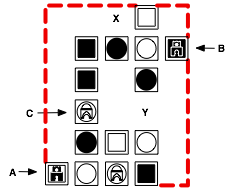
\includegraphics[scale=0.9]{slidetile.png}
\caption{Peças deslocáveis}
\label{fig:slidetile}
\end{figure}

A torre A pode mover a sua peça para a posição X, mas a torre B não pode (visto que teria de aumentar o tamanho do tabuleiro a meio da jogada para o fazer). A torre C apenas se pode deslocar para a posição Y, porque é a unica posição em que o tabuleiro continua todo conectado. A outra torre não se pode mexer.

\subsubsection{Passar a vez}

Basta não fazer nada e passar a vez ao outro jogador. Um jogador que não pode fazer nada é obrigado a passar.


\subsection{Fim do jogo}

Há três formas de ganhar o jogo. Uma já foi dita anteriormente (ter uma ilha completa). As outras duas são usadas principalmente para evitar empates e que os jogos durem demasiado tempo.

\subsubsection{Ilha completa}

Um jogador vence quando todas as peças restantes da sua cor, ou da sua forma, estão conectadas.
Se todas as peças de uma cor ou forma estão conectadas quando o tabuleiro é inicialmente construído, o jogador que colocar as torres deve inicalmente trocar duas peças cuja numeração no formato de jogo usado (ver figuras \ref{fig:syrtismajor} e \ref{fig:syrtisminor}) sejam seguidas. Por exemplo, trocar a peça 11 com a peça 12. Deve continuar a usar-se este método até que tal deixe de acontecer.

\subsubsection{Areias movediças}

Se um jogador afundar quatro peças sem o outro jogador ter afundado nenhuma, o segundo perde, sendo engolido pelas areias movediças.
Os jogadores devem controlar quantas peças afundaram desde que o outro jogador afundou a última peça.

\subsubsection{Iniciativa}

Esta regra existe para evitar empates. O jogo termina se alguma das seguintes situações ocorrer:

\begin{itemize}
\item Ambos os jogadores conseguem uma ilha completa ao mesmo tempo;
\item Ambos os jogadores passam a sua vez em jogadas consecutivas (ou seja, ambos passam duas vezes cada um);
\item Um jogador passa quatro vezes seguidas.
\end{itemize}

Em qualquer um dos casos, o último jogador a afundar uma peça ganha. Se nenhum dos jogadores tiver afundado uma peça, o jogador que jogou primeiro ganha.

\begin{figure}[h]
\centering
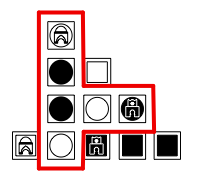
\includegraphics[scale=0.9]{win.png}
\caption{Uma situação em que o jogador branco ganhou ao completar uma ilha de círculos.}
\label{fig:win}
\end{figure}

%%%%%%%%%%%%%%%%%%%%%%%%%%
\section{Representação do Estado do Jogo}

O jogo será representado numa lista de listas de listas. As duas primeiras listas representarão o tabuleiro de jogo. A 3ª lista representará o conteúdo de cada quadrado do tabuleiro, utilizando o formato [Torre,Cor,Forma].

\begin{itemize}
\item \textbf{Torre:} Representa a existência ou não de uma torre no quadrado. Em caso afirmativo, utiliza a letra 'L' para representar uma torre branca, circular, e uma letra 'T' para uma torre preta, quadrangular.
\item \textbf{Cor:} Representa a cor da do quadrado. Se for preto, utiliza-se a letra 'P', se for branco utiliza-se a letra 'B'.
\item \textbf{Forma:} Representa a forma da peça do quadrado. Se for um círculo, usa-se a letra 'C', se for um quadrado usa-se a letra 'Q'.
\end{itemize}

Para todos os casos, a não existência do objeto implica a representação através de um espaço (' ').

Segue-se um exemplo de representação do board quando o jogo começa:

\begin{lstlisting}
beggining_board(Board) :- Board =
[	[[' ',' ',' '], [' ',' ',' '],[' ','B','C'], [' ','B','Q'],
	 [' ','B','Q'], [' ',' ',' '],[' ',' ',' ']],
	[[' ',' ',' '], [' ','P','Q'],[' ','P','C'], [' ','P','Q'],
 	 ['L','B','C'], [' ','P','C'], [' ',' ',' ']],
	[[' ','P','C'], [' ','B','Q'], ['L','B','C'], [' ','B','Q'],
	 [' ','P','Q'], [' ','B','C'], [' ','B','C']],
	[[' ','P','Q'], [' ','P','C'], [' ','P','C'], [' ',' ',' '],
	 ['T','B','Q'], [' ','B','Q'], [' ','B','C']],
 	[[' ','P','Q'], [' ','P','Q'], [' ','B','C'], [' ','P','C'],
 	 [' ','P','Q'], [' ','P','C'], [' ','B','Q']],
 	[[' ',' ',' '], ['T','B','Q'], [' ','P','Q'], [' ','B','C'],
 	 [' ','B','Q'], [' ','B','C'], [' ',' ',' ']],
 	[[' ',' ',' '], [' ',' ',' '], [' ','P','C'], [' ','P','C'],
 	 [' ','P','Q'], [' ',' ',' '], [' ',' ',' ']]].
\end{lstlisting}

Quando o jogo está a meio:

\begin{lstlisting}
middle_board(Board) :- Board =
[	[[' ',' ',' '], [' ',' ',' '], [' ',' ',' '], [' ',' ',' '],
	 [' ','B','Q'], [' ',' ',' '], [' ',' ',' ']],
 	[[' ',' ',' '], [' ',' ',' '], [' ','P','Q'], [' ','P','C'],
 	 [' ','B','C'], ['T','P','Q'], [' ',' ',' ']],
	[[' ',' ',' '], [' ',' ',' '], [' ','P','Q'], [' ',' ',' '],
	 [' ','P','Q'], [' ',' ',' '], [' ',' ',' ']],
	[[' ',' ',' '], [' ',' ',' '], ['L','B','C'], [' ',' ',' '],
	 [' ',' ',' '], [' ',' ',' '], [' ',' ',' ']],
 	[[' ',' ',' '], [' ',' ',' '], [' ','P','C'], [' ','B','Q'],
 	 [' ',' ',' '], [' ',' ',' '], [' ',' ',' ']],
 	[[' ',' ',' '], ['T','B','Q'], [' ','B','C'], ['L','B','C'],
 	 [' ','P','Q'], [' ',' ',' '], [' ',' ',' ']],
 	[[' ',' ',' '], [' ',' ',' '], [' ',' ',' '], [' ',' ',' '],
 	 [' ',' ',' '], [' ',' ',' '], [' ',' ',' ']]].
\end{lstlisting}

E quando o jogo acaba:

\begin{lstlisting}
end_board(Board) :- Board =
[	[[' ',' ',' '], [' ',' ',' '], [' ',' ',' '], [' ',' ',' '],
	 [' ',' ',' '], [' ',' ',' '], [' ',' ',' ']],
 	[[' ',' ',' '], [' ',' ',' '], [' ',' ',' '], [' ',' ',' '],
 	 [' ',' ',' '], [' ',' ',' '], [' ',' ',' ']],
	[[' ',' ',' '], [' ',' ',' '], ['L','B','C'], [' ',' ',' '],
	 [' ',' ',' '], [' ',' ',' '], [' ',' ',' ']],
	[[' ',' ',' '], [' ',' ',' '], [' ','P','C'], [' ','Q','B'],
	 [' ',' ',' '], [' ',' ',' '], [' ',' ',' ']],
 	[[' ',' ',' '], [' ',' ',' '], [' ','P','C'], [' ','B','C'],
 	 ['T','B','C'], [' ',' ',' '], [' ',' ',' ']],
 	[['L','B','Q'], [' ','B','C'], ['T','P','Q'], [' ','P','Q'],
 	 [' ','P','Q'], [' ',' ',' '], [' ',' ',' ']],
 	[[' ',' ',' '], [' ',' ',' '], [' ',' ',' '], [' ',' ',' '],
 	 [' ',' ',' '], [' ',' ',' '], [' ',' ',' ']]].
\end{lstlisting}

%Descrever a forma de representação do estado do %tabuleiro (tipicamente uma lista de listas), %com exemplificação em Prolog de posições %iniciais do jogo, posições intermédias e %finais, acompanhadas de imagens ilustrativas.


%%%%%%%%%%%%%%%%%%%%%%%%%%
\section{Visualização do Tabuleiro}

Para efeitos de demonstração, fizemos dois tabuleiros, um do tipo Syrtis Major e outro do tipo Syrtis Minor, \textit{hard-coded}. Para os obter, faz-se uma das seguintes chamadas:

\begin{lstlisting}
major_board(Board), display_board(Board).
\end{lstlisting}

ou

\begin{lstlisting}
minor_board(Board), display_board(Board).
\end{lstlisting}

As funções irão futuramente criar um tabuleiro aleatório com o formato especificado nas figuras \ref{fig:syrtismajor} e \ref{fig:syrtisminor} respetivamente.

Código da implementação (incluindo os dois tabuleiros \textit{hard-coded} ):

\lstinputlisting[language=Prolog]{../board.pl}

A figura \ref{fig:outputboard} mostra uma imagem com o output produzido.

\begin{figure}[h]
\centering
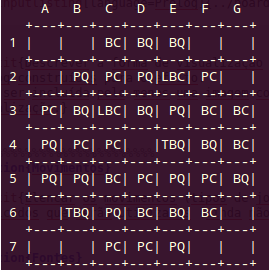
\includegraphics[scale=0.5]{outputboard.png}
\caption{Output produzido pelas chamadas a majorBoard e minorBoard}
\label{fig:outputboard}
\end{figure}


%%%%%%%%%%%%%%%%%%%%%%%%%%
\section{Movimentos}

Tal como já foi referido anteriormente na secção \ref{sec:actions}, existem 4 jogadas possíveis que um jogador pode fazer na sua jogada: mover uma torre, afundar uma peça, deslocar uma peça ou passar a vez. Apresentam-se 4 cabeçalhos para os predicados que serão utilizados para implementar estas acções:

\begin{lstlisting}

valid_slide(Board, StartRow, StartCol, FinalRow, FinalCol).
slide_tile(Board, StartRow, StartCol, FinalRow, FinalCol, FinalBoard).

valid_remove(Board,Row,Col).
remove_tile(Board,Row,Col,Board).

valid_move(Board, StartRow, StartCol, FinalRow, FinalCol).
move_tower(Board, StartRow, StartCol, FinalRow, FinalCol, FinalBoard).

pass(Board).

\end{lstlisting}

\section{Fontes}

http://www.playsyrtis.com/interstate/

\end{document}
